\section{平面问题的直角坐标解答}
\subsection{逆解法}
\subsubsection{含义}
所谓逆解法,就是先设定各种形式的满足双调和方程的应力函数,然后利用应力函数计算各个应力分量,再根据应力边界条件反算边界上对应的面力,从而得知所设定的应力函数可以解决什么样的应力问题。
\subsubsection{步骤}
\[\begin{array}{c}
\text{设定}\Phi\\
\text{满足}\nabla ^4\Phi =0\\
\end{array}\rightarrow \text{求出应力分量}\xrightarrow{\text{代入边界条件}}\text{反推面力}\rightarrow \text{得出可解决的应力问题}\]
\subsubsection{唯一性定理}
在洽定载荷作用下,处于平衡状态的弹性体,其内部各点的应力,应力解是唯一的,如果物体的整体刚体位移收到约束,则位移解也是位移的。
\subsubsection{多项式解答}
\begin{enumerate}
	\item 多项式应力函数$\varPhi \left( x,y \right) $都性质
	\begin{itemize}
		\item 多项式次数$n<4$时,则系数可以任意选取,总满足相容方程。
		\item 多项式次数$n\geqslant 4$时,则系数需满足一定的条件,才能满足相容方程。
		\item 多项式次数越高,则系数间需满足的条件越多。
	\end{itemize}
	\item 一次多项式:对应于无体力和无应力状态的自然状态;任意应力函数$\varPhi \left( x,y \right) $加上或减去一个一次多项式,对应力无影响。
	\item 二次多项式:对应均匀应力状态,即全部应力分量为常量。
	\item 三次多项式:对应线性分布的应力。
	\item 用多项式构造应力函数$\varPhi \left( x,y \right) $,一般只能解决简单直线应力边界问题。
\newpage
\begin{example}
	设图中所示的矩形长梁($l\geqslant h$),试考察应力函数$\varPhi =\frac{F}{2h^3}xy\left( 3h^2-4y^2 \right) $能解决什么样的受力问题?
\end{example}
\end{enumerate}
\begin{figure*}[!h]
\centering
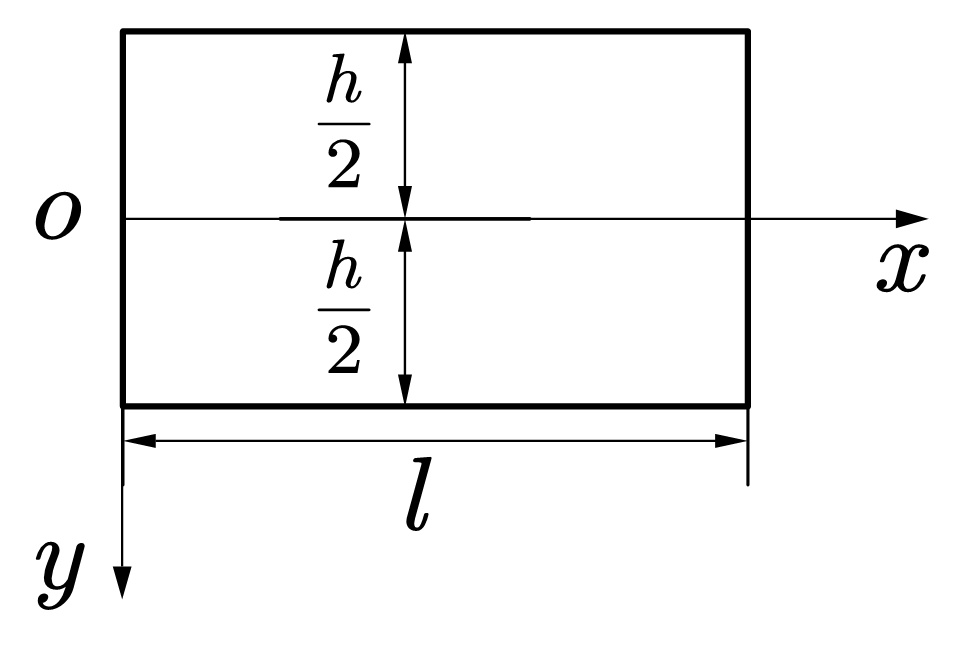
\includegraphics[scale=0.4]{figure/3-1.png}
\end{figure*}
	\begin{remark}
		按照逆解法:
		\begin{enumerate}
			\item 将$\varPhi$代入相容方程,$\nabla ^4\Phi =0$满足。
			\item 由$\varPhi$求出应力分量:\[\begin{cases}
			\sigma _x=\frac{\partial ^2\varPhi}{\partial y^2}=-\frac{12Fxy}{h^3}\\
			\sigma _y=\frac{\partial ^2\varPhi}{\partial x^2}=0\\
			\tau _{xy}=-\frac{\partial ^2\varPhi}{\partial x\partial y}=\frac{3F}{2h}\\
			\end{cases}\]
			\item 由边界形状和应力分量反推边界上的应力。\\
			主要边界(大边界):$y=\pm \frac{h}{2},\sigma _y=0,\tau _{xy}=0\text{。}$\\
			因此:在$y=\pm \frac{h}{2}$的边界面上,无任何面力作用。即:$\bar{f}_x=\bar{f}_y=0$\\
			次要边界(小边界)$x=0 or\,\,l$上:\\
			左端:\[\begin{cases}
			\bar{f}_x=-\left( \sigma _x \right) _{x=0}=0\\
			\bar{f}_y=-\left( \tau _{xy} \right) _{x=0}=\frac{3F}{2h}\left( 1-\frac{4}{h^2}y^2 \right)\\
			\end{cases}\]
			右端:\[\begin{cases}
			\bar{f}_x=-\left( \sigma _x \right) _{x=l}=-\frac{12Fl}{h^3}y\\
			\bar{f}_y=-\left( \tau _{xy} \right) _{x=l}=-\frac{3F}{2h}\left( 1-\frac{4}{h^2}y^2 \right)\\
			\end{cases}\]\\
		\end{enumerate}
		\centerline{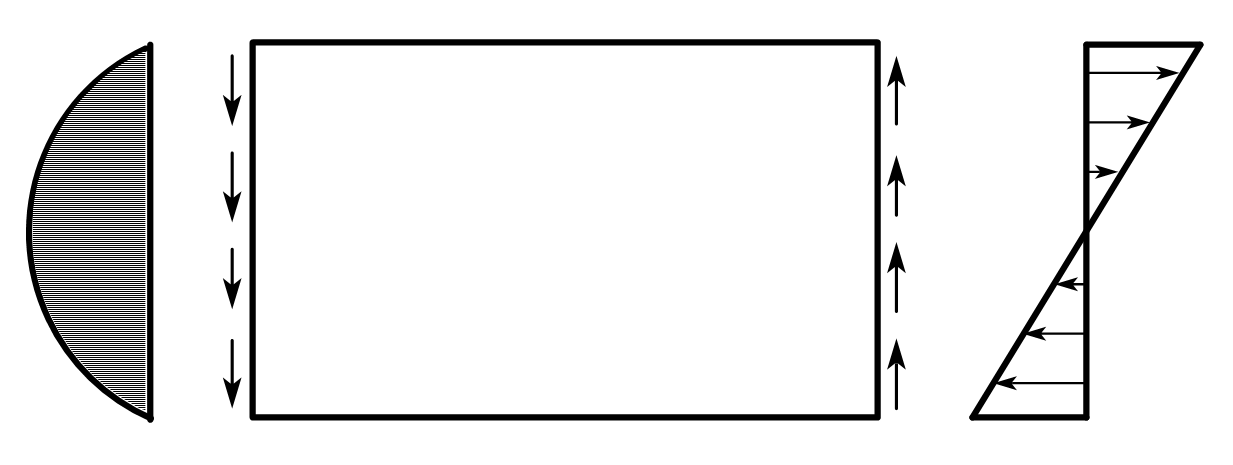
\includegraphics[scale=0.6]{figure/3-2.png}}
	\end{remark}
\begin{example}
	不计体力,应力函数$\varPhi =\frac{q}{6l}x^3$能解决什么样的受力问题?
\end{example}
\centerline{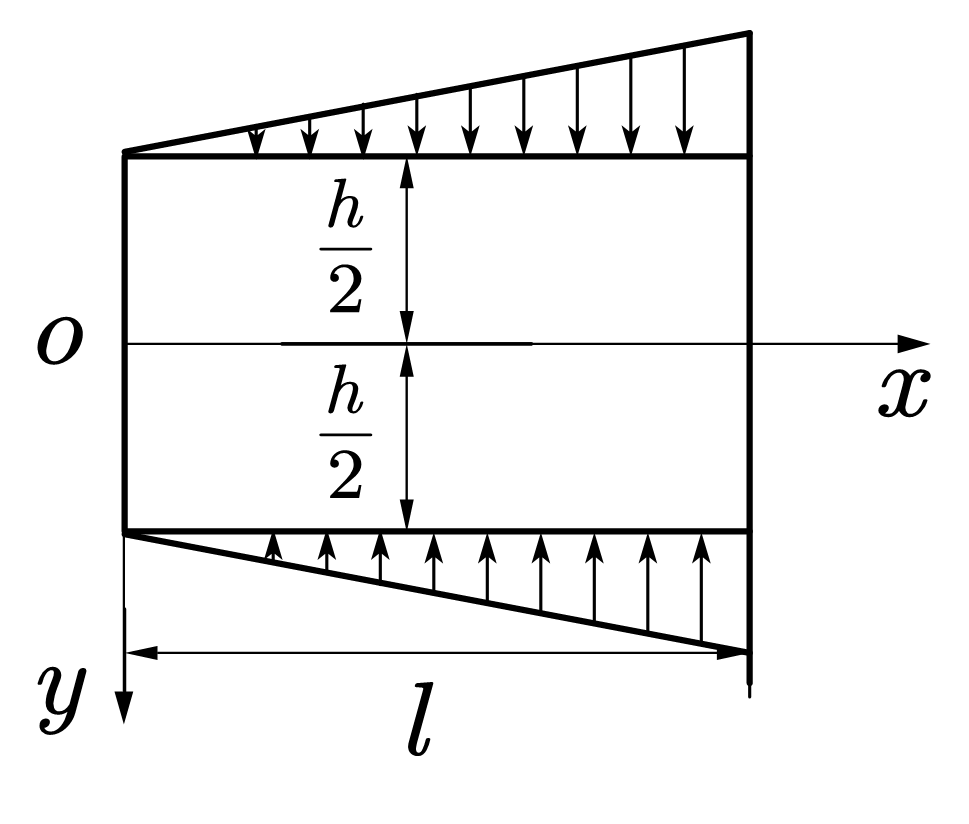
\includegraphics[scale=0.6]{figure/3-4.png}}

\begin{remark}
	按照逆解法:
	\begin{enumerate}
		\item 代入相容方程,最高次为3次,故满足。
		\item 由$\varPhi $求出应力分量:\[\begin{cases}
		\sigma _x=0\\
		\sigma _y=\frac{q}{l}x\\
		\tau _{xy}=0\\
		\end{cases}\]
		\item 边界条件:\\
		上边界:\[\bar{f}_y=-\sigma _y=-\frac{q}{l}x\]
		下边界:\[\bar{f}_y=-\sigma _y=\frac{q}{l}x\]
		左边界:\[\begin{cases}
		\bar{f}_x=-\left( \sigma _x \right) _{x=0}=0\\
		\bar{f}_y=-\left( \tau _{xy} \right) _{x=0}=0\\
		\end{cases}\]
		右边界:\[\begin{cases}
		\bar{f}_x=-\left( \sigma _x \right) _{x=l}=0\\
		\bar{f}_y=-\left( \tau _{xy} \right) _{x=l}=0\\
		\end{cases}\]
		因此在左右边界上无任何面力作用。
	\end{enumerate}
	
\end{remark}



\subsection{矩形梁的纯弯曲}
\centerline{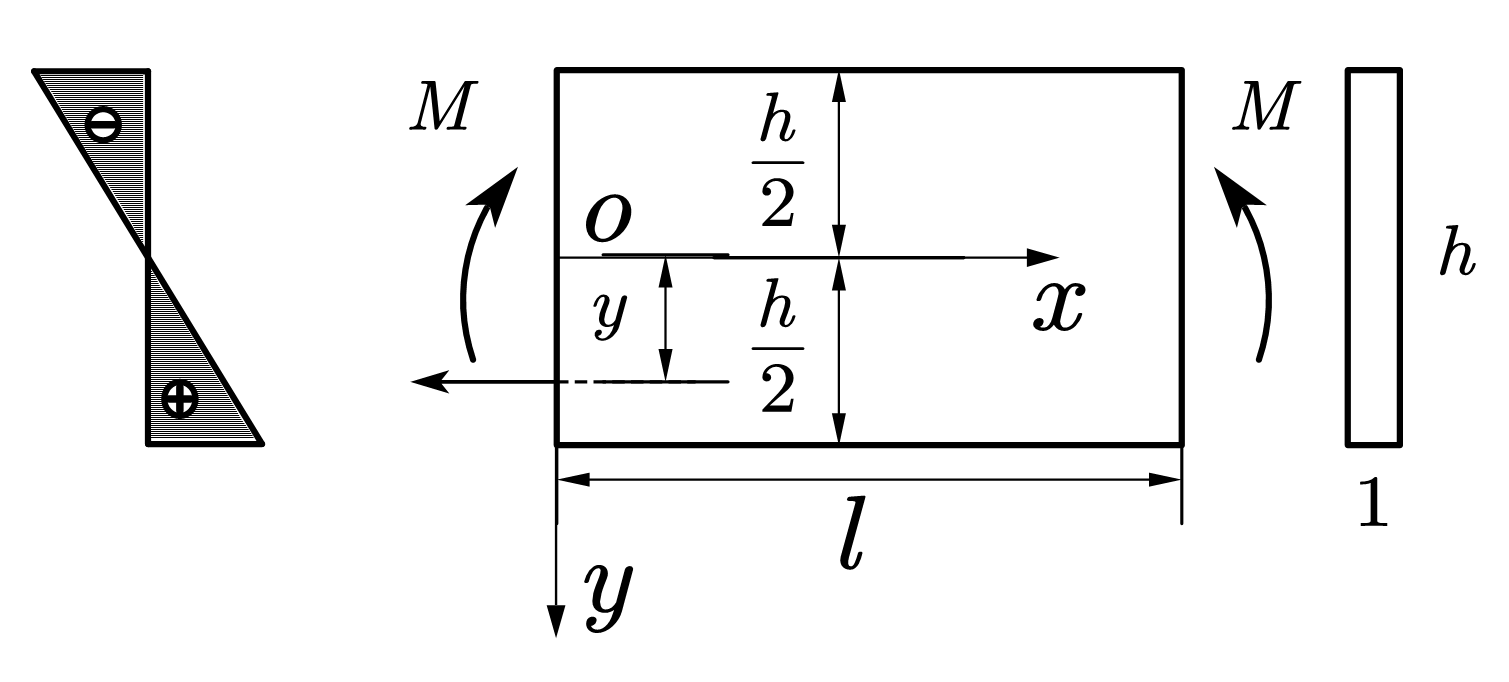
\includegraphics[scale=0.6]{figure/3-3.png}}
应力函数:\[\varPhi =ay^3\]
相应的应力分量:\[\sigma _x=6ay,\sigma _y=0,\tau _{xy}=\tau _{yx}=0\]
由圣维南原理可得:\[\int_{-\frac{h}{2}}^{\frac{h}{2}}{\sigma _xydy}=M\Longrightarrow a=\frac{2M}{h^3}\]
于是应力函数又可以写为:\[\sigma _x=\frac{M}{I}y,\sigma _y=0,\tau _{xy}=\tau _{yx}=0\]
\begin{enumerate}
	\item 弹性力学的解答和材料力学的解答完全一致。
	\item 只有组成两端力偶的法面面力是线性分布,在截面中处为零时,本节所求的解才是完全精确的。如果梁端的面力是按照其他方式分布的,解答是有误差的,根据圣维南原理,只有梁两端附近小区域有显著误差,在远端误差可以忽略不计。
\end{enumerate}
\subsection{位移分量的求出}
将应力分量代入物理方程,得到应变分量,再代入几何方程,得到位移分量的微分方程组,求解即可得到位移分量。其中结合位移限制条件可以完全确定出位移分量的表达式。
\[\text{应力分量}\xrightarrow{\text{物理方程}}\text{应变分量}\xrightarrow{\text{几何方程}}\text{位移方程组}\xrightarrow{\text{位移边界条件}}\text{积分常数}\longrightarrow \text{位移分量}\]
\subsection{半逆解法}
求解步骤:
\begin{enumerate}
	\item 根据弹性体的边界形状和受力情况,假定部分或全部应力分量的函数形式。
	\item 根据应力分量和压力函数之间的关系,反推应力函数的函数形式。
	\item 由相容方程的满足来确定应力函数中的待定项。
	\item 根据应力分量和应力函数之间的关系,求出全部应力分量的具体表达式。
	\item 根据边界条件,确定待定常数。
\end{enumerate}
\begin{example}
	设有矩形截面的长竖柱,密度为$\rho$,在一边侧面上受有均布面力$q$,如图所示,试求应力分量。
\end{example}
\centerline{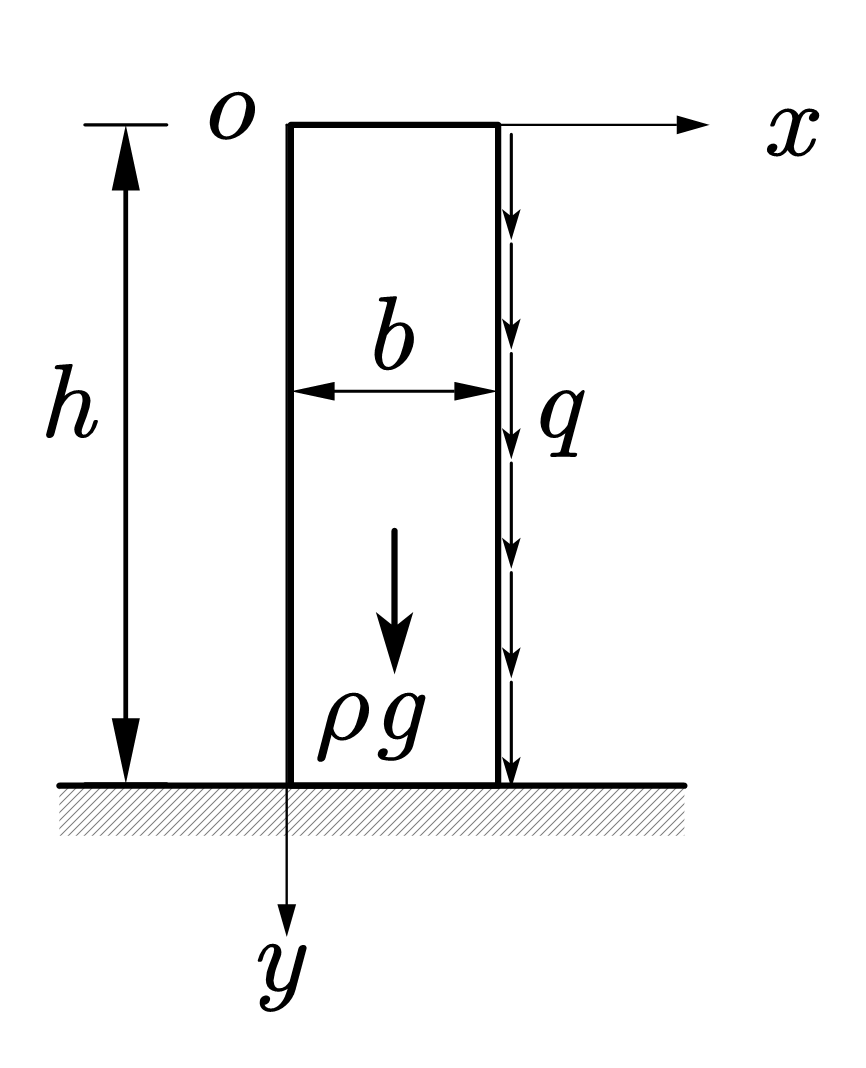
\includegraphics[scale=0.7]{figure/3-5.png}}
\begin{remark}
	\quad
	\begin{enumerate}
		\item 假设某个应力分量的函数形式。\\
		分析:只有$y$向体力$f_y=\rho g$面力$\left( \bar{f}_y \right) _{x=b}=q$\\
		突破点:假设在整个长柱内:$\sigma _x=0$
		\item 根据应力分量导出应力函数的表达式\[\sigma _x=\frac{\partial ^2\varPhi}{\partial y^2}\rightarrow \frac{\partial ^2\varPhi}{\partial y^2}=0\rightarrow \frac{\partial \varPhi}{\partial y}=f\left( x \right) \rightarrow \varPhi =yf\left( x \right) +f_1\left( x \right) \]
		\item 由相容方程求解出应力函数:\[\begin{cases}
		\frac{\partial ^4\varPhi}{\partial x^4}+2\frac{\partial ^4\varPhi}{\partial x^2\partial y^2}+\frac{\partial ^4\varPhi}{\partial y^4}=0\\
		\frac{\partial ^4\varPhi}{\partial y^4}=0\\
		\frac{\partial ^4\varPhi}{\partial x^2\partial y^2}=0\\
		\end{cases}\Longrightarrow \frac{\partial ^4\varPhi}{\partial x^4}=y\frac{d^4f\left( x \right)}{dx^4}+\frac{d^4f_1\left( x \right)}{dx^4}=0\]
		\[\begin{cases}
		\frac{d^4f\left( x \right)}{dx^4}=0\Longrightarrow f\left( x \right) =Ax^3+Bx^2+Cx\\
		\frac{d^4f_1\left( x \right)}{dx^4}=0\Longrightarrow f_1\left( x \right) =Dx^3+Ex^2\,\, \left( \text{省略一}次\text{项} \right)\\
		\end{cases}\]
		\item 由应力函数求解应力分量\[\varPhi =y\left( Ax^3+Bx^2+Cx \right) +Dx^3+Ex^2,f_x=0;f_y=\rho g\]
		\[\begin{cases}
		\sigma _x=\frac{\partial ^2\varPhi}{\partial y^2}-f_xx=0\\
		\sigma _y=\frac{\partial ^2\varPhi}{\partial x^2}-f_yy=y\left( 6Ax+2B \right) +6Dx+2E-\rho gy\\
		\tau _{xy}=-\frac{\partial ^2\varPhi}{\partial x\partial y}=-\left( 3Ax^2+2Bx+C \right)\\
		\end{cases}\]
		\item 由应力边界条件确定积分常数
		\begin{enumerate}
			\item 左右边界(主要边界):\[\begin{cases}
			\sigma _x=\frac{\partial ^2\varPhi}{\partial y^2}-f_xx=0\\
			\sigma _y=\frac{\partial ^2\varPhi}{\partial x^2}-f_yy=y\left( 6Ax+2B \right) +6Dx+2E-\rho gy\\
			\tau _{xy}=-\frac{\partial ^2\varPhi}{\partial x\partial y}=-\left( 3Ax^2+2Bx+C \right)\\
			\end{cases}\]
			\item 上边界(次要边界),应用圣维南原理:
			\[\begin{cases}
			\int_0^b{\left( \sigma _y \right) _{y=0}dx=0}\\
			\int_0^b{\left( \sigma _y \right) _{y=0}dx}=0\\
			\int_0^b{\left( \tau _{xy} \right) _{y=0}dx}=0\\
			\end{cases}\Longrightarrow \begin{cases}
			3Db+2E=0\\
			2Db+E=0\\
			Ab^2+6Bb+C=0\\
			C=0\\
			3Ab^2+2Bb+C=-q\\
			\end{cases}\Longrightarrow \begin{cases}
			A=-\frac{q}{b^2}\\
			B=\frac{q}{b}\\
			C=D=E=0\\
			\end{cases}\]
		\end{enumerate}
	最终得到应力分量表达式\[\begin{cases}
	\sigma _x=0\\
	\sigma _y=\frac{2q}{b}y\left( 1-\frac{3}{b} \right) -\rho gy\\
	\tau _{yx}=\frac{3q}{b^2}x^2-\frac{2q}{b}x\\
	\end{cases}\]
	\end{enumerate}
\end{remark}
\begin{example}
设单位厚度的悬臂梁在左端受到集中力和力矩的作用,体力可以不计。如图示,设应力函数$\varPhi =Axy+By^2+Cy^3+Dxy^3$,求解应力分量。
\end{example}
\centerline{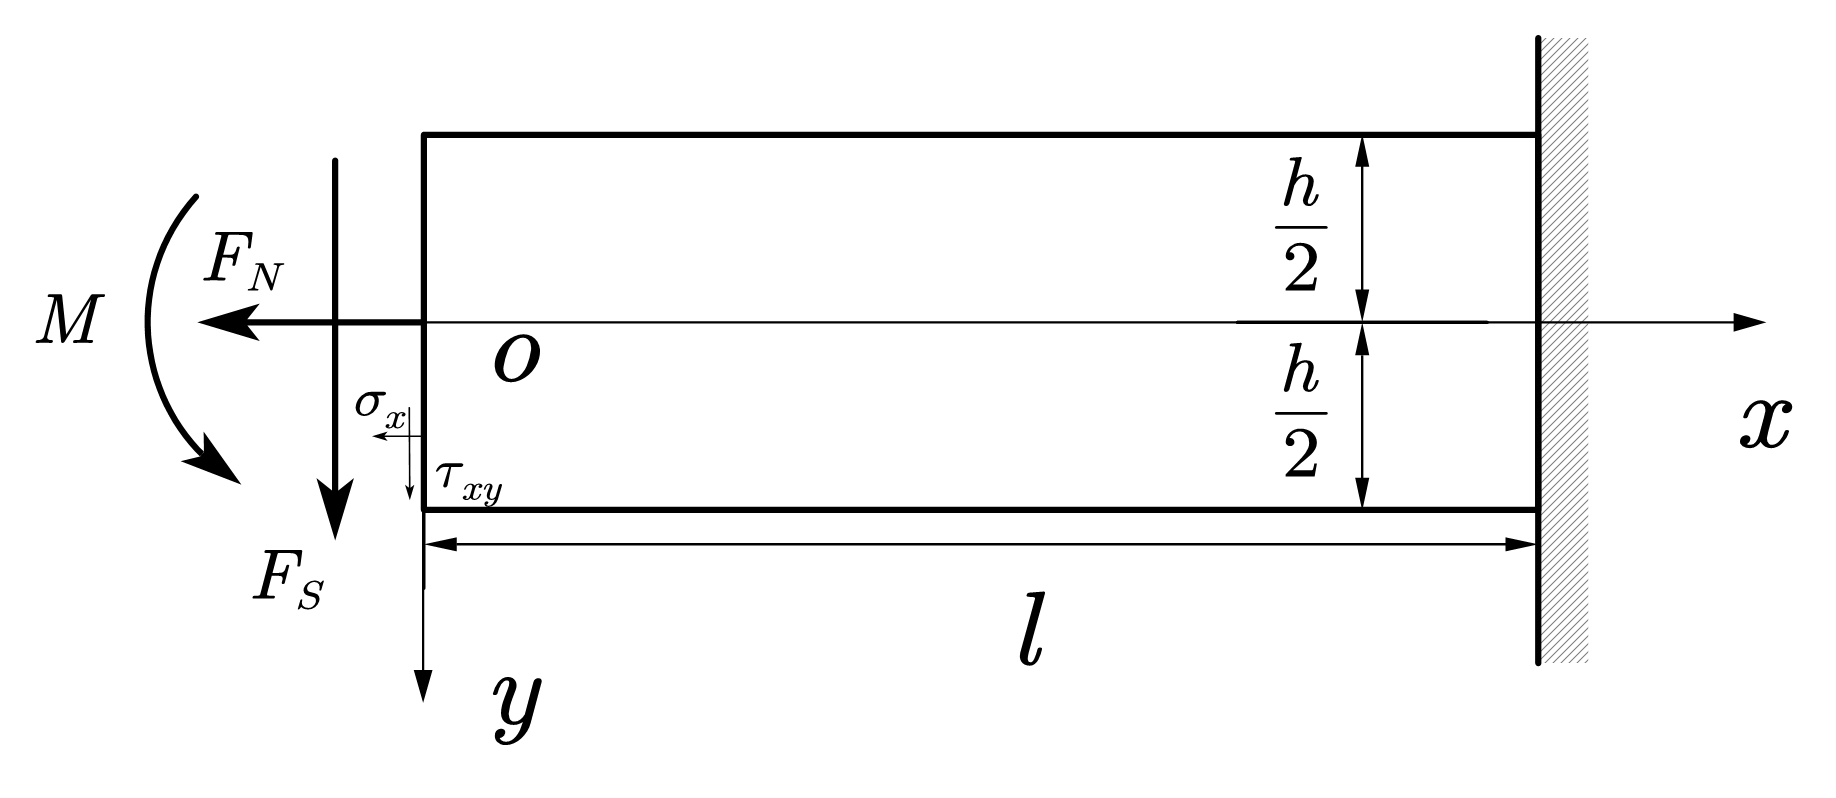
\includegraphics[scale=0.6]{figure/3-6.png}}
\begin{remark}
\begin{enumerate}
	\quad
	\item 校核相容方程$\nabla ^4\varPhi =0$,满足。
	\item 求应力分量,无体力时\[\begin{cases}
	\sigma _x=\frac{\partial ^2\varPhi}{\partial y^2}=2B+6Cy+6Dxy\\
	\sigma _y=\frac{\partial ^2\varPhi}{\partial x^2}=0\\
	\tau _{xy}=-\frac{\partial ^2\varPhi}{\partial x\partial y}=-\left( A+3Dy^2 \right)\\
	\end{cases}\]
	\item 校核主要边界条件:\[\begin{cases}
	\left( \sigma _y \right) _{y=\pm \frac{h}{2}}=0 \text{满足}\\
	\left( \tau _{xy} \right) _{y=\pm \frac{h}{2}}\rightarrow A+\frac{3}{4}Dh^2=0\\
	\end{cases}\]
	\item 校核次要边界,应用圣维南原理\[\begin{cases}
	\int_{-\frac{h}{2}}^{\frac{h}{2}}{\left( \sigma _x \right) _{x=0}dy}=-F_N\rightarrow B=-\frac{F_N}{2h}\\
	\int_{-\frac{h}{2}}^{\frac{h}{2}}{y\left( \sigma _x \right) _{x=0}dy}=-M\rightarrow C=-\frac{2M}{h^3}\\
	\int_{-\frac{h}{2}}^{\frac{h}{2}}{\left( \tau _{xy} \right) _{x=0}dy}=-F_S\rightarrow \begin{cases}
	A+\frac{Dh^3}{4}=F_S\\
	A+\frac{3Dh^2}{4}=0\\
	\end{cases}\Longrightarrow \begin{cases}
	A=\frac{3F_S}{2}\\
	D=-\frac{2F_S}{h^3}\\
	\end{cases}\\
	\end{cases}\]
	故得:\[\begin{cases}
	\sigma _x=-\frac{F_N}{h}-\frac{12M}{h^3}y-\frac{12F_S}{h^3}xy\\
	\sigma _y=0\\
	\tau _{xy}=-\frac{3F_S}{2h}\left( 1-4\frac{y^4}{h^2} \right)\\
	\end{cases}\]
\end{enumerate}
\end{remark}
\begin{example}
	挡承强的密度为$\rho$,厚度为$b$,如图示,水的密度为$\rho_2$,试求应力分量。
\end{example}
\centerline{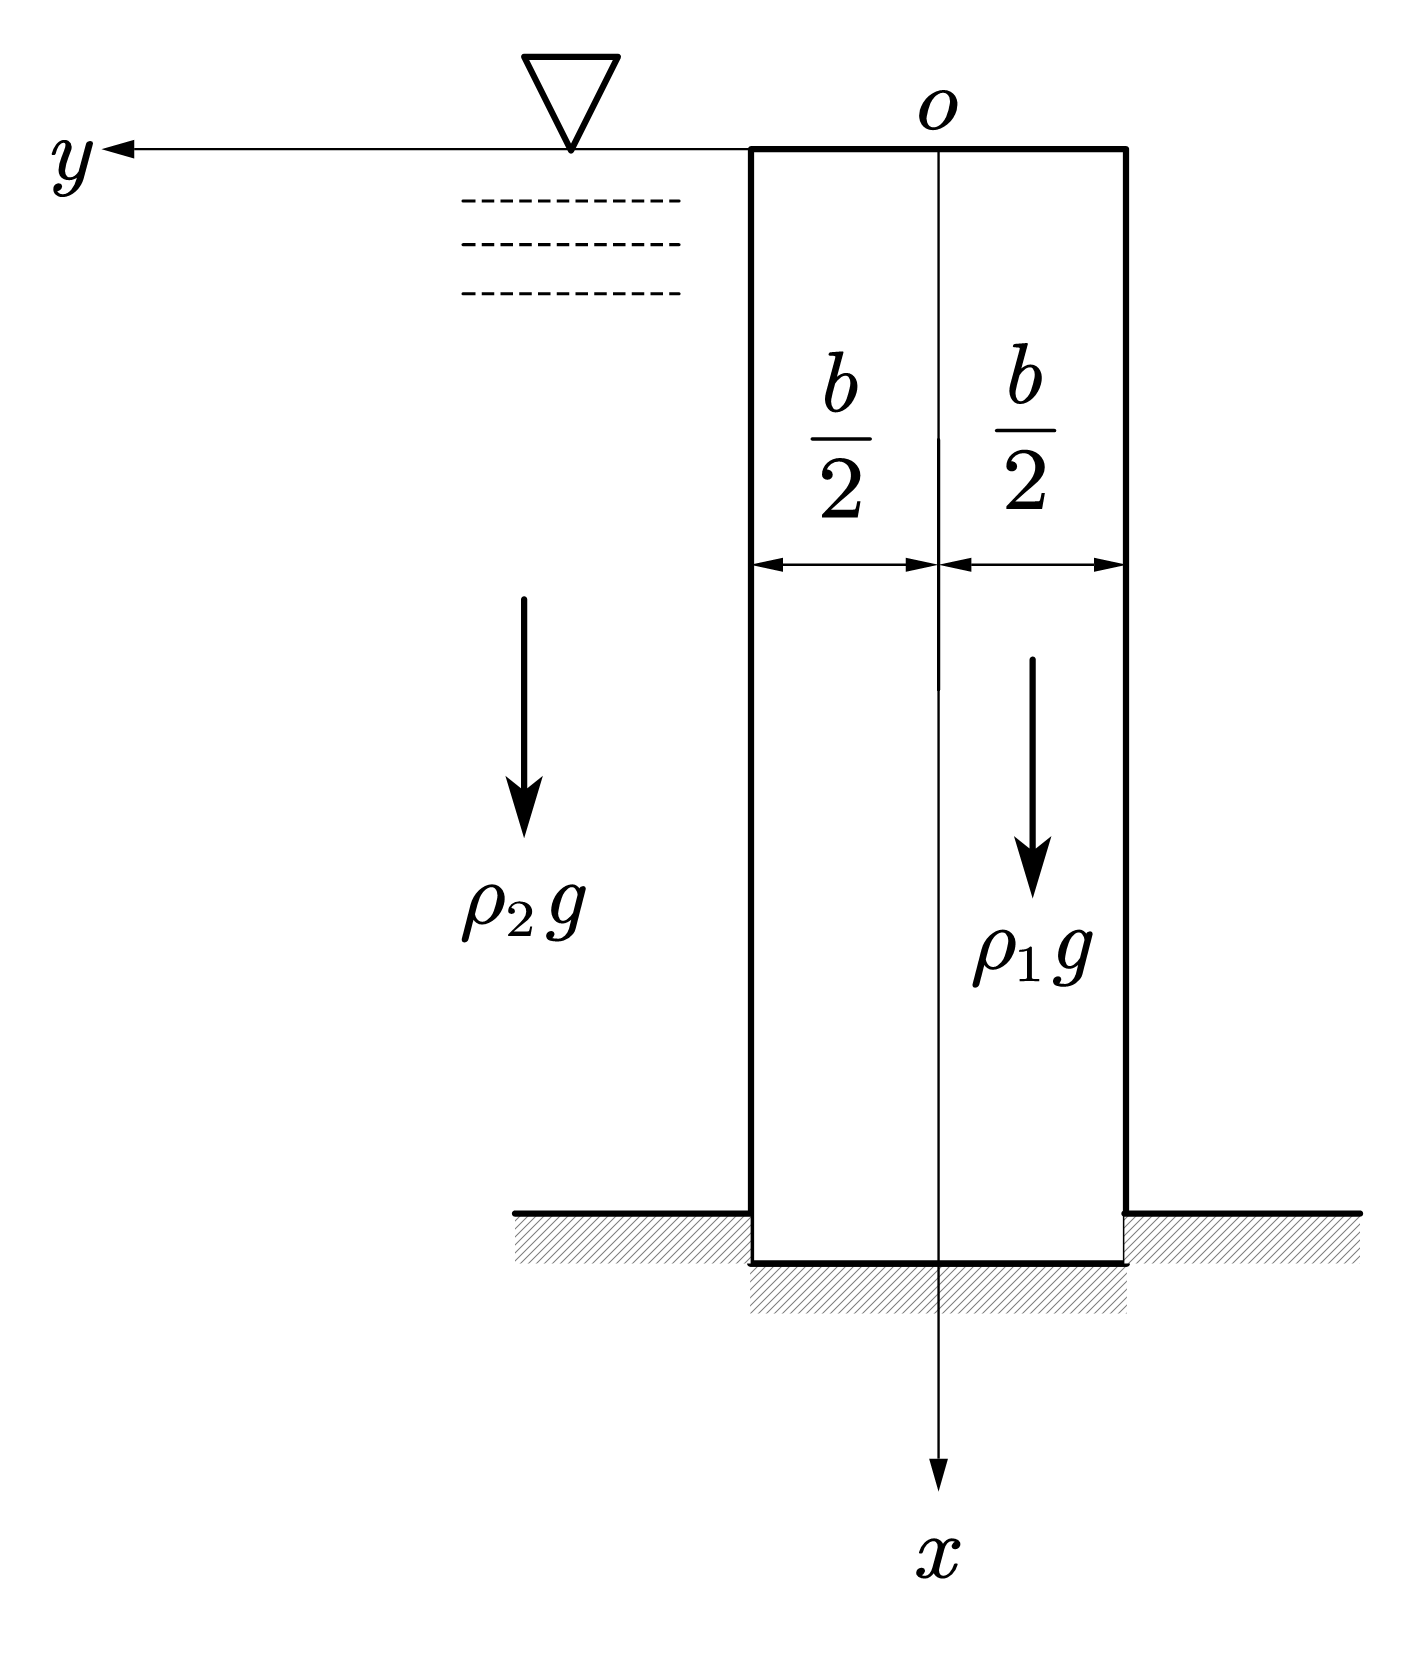
\includegraphics[scale=0.4]{figure/3-7.png}}
\begin{remark}
用半逆解法解
\begin{enumerate}
	\item 假设应力分量的应力函数形式,因为在$y=-\frac{b}{2}$边界上$\sigma _y=0$,而在$y=\frac{b}{2}$边界上$\sigma _y=-\rho _2gx$;所以可假设在区域内$\sigma _y$是按照一次式变化,即\[\sigma _y=xf\left( y \right) \]
	\item 根据应力分量导出应力函数的表达式\[\sigma _y=\frac{\partial ^2\varPhi}{\partial x^2}=xf\left( y \right) \Longrightarrow \varPhi =\frac{x^3}{6}f\left( y \right) +xf_1\left( y \right) +f_2\left( y \right) \]
	\item 根据相容方程求解应力函数\[\frac{x^3}{6}\frac{d^4f\left( y \right)}{dy^4}+x\frac{d^4f_1\left( y \right)}{dy^4}+\frac{d^4f_2\left( y \right)}{dy^4}+2x\frac{d^2f\left( y \right)}{dy^2}=0\]
	\[\begin{cases}
	\frac{d^4f}{dy^4}=0\Longrightarrow f=Ay^3+By^2+Cy+D\\
	\frac{d^4f_1}{dy^4}+2\frac{d^2f}{dy^2}=0\Longrightarrow f_1=-\frac{A}{10}y^5-\frac{B}{6}y^4+Gy^3+Hy^2+Iy\\
	\frac{d^4f_2}{dy^4}=0\Longrightarrow f_2=Ey^3+Fy^2\\
	\end{cases}\]
	\[\varPhi =\frac{1}{6}x^3\left( Ay^3+By^2+Cy+D \right) +x\left( -\frac{A}{10}y^5-\frac{B}{6}y^4+Gy^3+Hy^2+Iy \right) +Ey^3+Fy^2\]
	\[\]
	\item 求出应力分力量\[\begin{cases}
	\sigma _x=x^3\left( Ay+\frac{B}{3} \right) +x\left( -2Ay^3-2By^2+6Gy^3+2H \right) +6Ey+2F-\rho _1gx\\
	\sigma _y=x\left( Ay^3+By^2+Cy+D \right)\\
	\tau _{xy}=-\frac{x^2}{2}\left( 3Ay^2+2By+C \right) +\left( \frac{A}{2}y^4+\frac{3B}{3}y^3-3Gy^2-2Hy-I \right)\\
	\end{cases}\]
	\item 由应力边界条件确定积分常数
	主要边界(左、右)必须精确满足边界条件:\[\left( \sigma _y \right) _{y=\frac{b}{2}}=-\rho _2gx;\left( \sigma _y \right) _{y=-\frac{b}{2}}=0;\left( \tau _{xy} \right) _{y=\frac{b}{2}}=0;\left( \tau _{xy} \right) _{y=-\frac{b}{2}}=0\]
	得:\[\begin{cases}
	A\frac{b^3}{8}+B\frac{b^2}{4}+C\frac{b}{2}+D=-\rho _2x\\
	-A\frac{b^4}{8}+B\frac{b^2}{4}-C\frac{b}{2}+D=0\\
	A\frac{3}{4}b^2\pm Bb+C=0\\
	A\frac{b^4}{32}\pm B\frac{b^3}{12}-G\frac{3}{4}b^2\pm Hb-I=0\\
	\end{cases}\]
	解得:\[\begin{cases}
	A=\frac{2}{b^3}\rho _2g\\
	B=0\\
	C=-\frac{3}{2b}\rho _2g\\
	D=-\frac{1}{2}\rho _2g\\
	H=0\\
	I=\frac{b}{16}\rho _2g-\frac{3b^2}{4}G\\
	\end{cases}\]
	次要边界(柱的上端),应用圣维南原理:\[\int_{-\frac{b}{2}}^{\frac{b}{2}}{\left( \sigma _x \right) _{x=0}dy=0},\int_{-\frac{b}{2}}^{\frac{b}{2}}{\left( \sigma _x \right) ydy=0},\int_{-\frac{b}{2}}^{\frac{b}{2}}{\left( \tau _{xy} \right) _{x=0}dy}=0\]
	解得:\[\begin{cases}
	F=E=0\\
	I=\frac{b}{80}\rho _2g-\frac{b^4}{4}G\\
	\end{cases}\]
	\item 最终应力分量表达
	\[\begin{cases}
	\sigma _x=\frac{2\rho _2g}{b^3}x^3y+\frac{3\rho _2g}{5b}xy-\frac{4\rho _2g}{b^3}xy^3-\rho _1gx\\
	\sigma _y=\rho _2gx\left( 2\frac{y^3}{b^3}-\frac{2y}{3b}-\frac{1}{2} \right)\\
	\tau _{xy}=-\rho _2gx^2\left( 3\frac{y^2}{b^3}-\frac{3}{4b} \right) -\rho _2gy\left( -\frac{y^3}{b^3}+\frac{3y}{10b}-\frac{b}{80y} \right)\\
	\end{cases}\]
\end{enumerate}
\end{remark}
\begin{example}
	已知:
	\begin{enumerate}
		\item $\varPhi =Ay^2\left( a^2-x^2 \right) +Bxy+C\left( x^2+y^2 \right) $
		\item $\varPhi =Ax^4+Bx^3y+Cx^2y^2+Dxy^2+Ey^4$
	\end{enumerate}
\end{example}
\begin{remark}
	\quad
	\begin{enumerate}
		\item 代入相容方程,$A=0$时才可能是应力函数。
		\item 代入相容方程,必须满足$3\left( A+E \right) +C=0$时才可能是应力函数。
	\end{enumerate}
\end{remark}